\documentclass{article}
\usepackage{blindtext}
\usepackage[utf8]{inputenc}
\usepackage{graphicx}
\usepackage{multicol}
\usepackage{listings}
\author{Ruben Van Assche}
\title{Orthangonale Functies - Oefening 6}
 
\begin{document}
 \maketitle
 \begin{flushleft}
\section{Chebychev Veeltermen}
 
In het eerste deel van de oefening wordt gevraagd om de Chebychev veeltermen $T_{4}(x)$ en $T_{7}(x) $ te berekenen.  Dit kan via de recursieve formule:
\newline

$ T_{0}(x) = 1$

$ T_{1}(x) = x$

$ T_{i+1}(x) = 2xT_{i}(x) - T_{i-1}(x)$
\newline

Hierdoor bekomen we na wat rekenwerk:
\newline

$ T_{0}(x) = 1$

$ T_{1}(x) = x$

$ T_{2}(x) = 2x^{2} - 1$

$ T_{3}(x) = 4x^{3} - 3x$

$ T_{4}(x) = 8x^{4} - 8x^{2} + 1$

$ T_{5}(x) = 16x^{5} - 20x^{3} + 5x$

$ T_{6}(x) = 32x^{6} - 48x^{4} + 18x^{2} - 1$

$ T_{7}(x) = 64x^{7} - 112x^{5} + 56x^{3} - 7x$
\section{Integralen verifieren}
 
Het tweede deel van de oefening vraagt om enkele integralen met chebychev veeltermen uit te rekenen en te controleren of deze uitkomsten overeenkomen met de gegeven uitkomsten.
\newline

De integralen zijn van de vorm:
\newline

$ \int_{-1}^{1}  \frac{T_{i}(X)T_{j}(X)}{\sqrt{1-x^{2}}} dx $
\newline

Nu is een mogelijke oplossing simpel: we vullen de chebychev veeltermen in de intergraal in. Vervolgens bekomen we een integraal die we niet zo snel kunnen integreren waardoor we dus numerieke integratie zullen moeten uitvoeren om de uitkomst van de integraal op het interval [-1, 1] te weten. Dit zal veel rekenwerk vereisen en dat willen we beperken
\newline

Nu is het ook mogelijk om de chebychev veeltermen te herschrijven, een compactere vorm van de chebychev veelterm is:
\newline

$T_{i}(x) = cos(i*arccos(x))$
\newline

Wanneer we deze compactere vorm gebruiken is het veel makkelijker deze integralen op te lossen.
\newline

\textbf{1. Integraal}
$ \int_{-1}^{1}  \frac{T_{0}(X)T_{1}(X)}{\sqrt{1-x^{2}}} dx = 0 $
\newline

Vermits we hier nog met een lage graad van de chebychev veelterm werken, zullen we het recursief voorschrift gebruiken inplaats van de compactere vorm, wanneer we dan de veeltermen invullen verkijgen we:
\newline

$ \int_{-1}^{1}  \frac{x}{\sqrt{1-x^{2}}} dx $
\newline

Wanneer we hierbij een subsititutie doen met $u = 1 - x^{2} $ en dus $ du = -2x $
\newline

$ -\frac{1}{2} \int_{-1}^{1}  \frac{1}{\sqrt{u}} du $
\newline

$ =  -\frac{1}{2} [ 2\sqrt{u} ]^{1}_{-1} $
\newline

$ =  [-\sqrt{1 - x^{2} } ]^{1}_{-1} $
\newline

Dit leidt dan tot:
\newline

$ -\sqrt{1 - 1^{2} } + \sqrt{1 - (-1)^{2} } = 0 $
\newline


\textbf{2. Integraal}
$ \int_{-1}^{1}  \frac{T_{4}(X)T_{7}(X)}{\sqrt{1-x^{2}}} dx = 0 $
\newline

Hierbij zullen we wel de compactere vorm van het chebychev polynoom gebruiken:
\newline

$ \int_{-1}^{1}  \frac{ cos(4cos^{-1}(x)) * cos(7cos^{-1}(x)) }{\sqrt{1-x^{2}}} dx = 0 $
\newline

Wanneer we hierbij een substitutie doen $u = cos^{-1}(x) $ en dus $ du = \frac{-1}{\sqrt{1-x^{2}}} $
\newline

$ = - \int_{-1}^{1}  cos(4u) * cos(7u)  du $
\newline

D.m.v. de trigoniometrie weten we $ cos(\alpha)*cos(\beta) = \frac{1}{2}(cos(\alpha - \beta) + cos(\alpha + \beta))$
\newline

$ = -\frac{1}{2} \int_{-1}^{1}  cos(3u) + cos(11u)  du $
\newline

$ = -\frac{1}{2} \int_{-1}^{1}  cos(3u) du -\frac{1}{2} \int_{-1}^{1} + cos(11u)  du $
\newline

$ = [-\frac{1}{6} sin(3u) - \frac{1}{22} sin(11u)]^{1}_{-1} $
\newline

$ = [-\frac{1}{6} sin(3cos^{-1}(x)) - \frac{1}{22} sin(11cos^{-1}(x))]^{1}_{-1} $
\newline

$ = -\frac{1}{6} sin(3cos^{-1}(1)) - \frac{1}{22} sin(11cos^{-1}(1)) + \frac{1}{6} sin(3cos^{-1}(-1)) + \frac{1}{22} sin(11cos^{-1}(-1)) $
\newline

$ = 0 $
\newline

\textbf{3. Integraal}
$ \int_{-1}^{1}  \frac{T_{4}(X)^{2}}{\sqrt{1-x^{2}}} dx = \frac{\pi}{2} $
\newline

Opnieuw maken we gebruik van de compactere chebychev vorm.
\newline

$ \int_{-1}^{1}  \frac{ cos(4cos^{-1}(x))^{2} }{\sqrt{1-x^{2}}} dx $
\newline

Wanneer we hierbij een substitutie doen $u = 4cos^{-1}(x) $ en dus $ du = \frac{-4}{\sqrt{1-x^{2}}} $
\newline

$ = -\frac{1}{4} \int_{-1}^{1}   cos(u)^{2} du $
\newline

Uit de trigoniometrie weten we dat $cos(x)^{2} = \frac{1}{2}(cos(2x) + 1)$
\newline

$ = -\frac{1}{4} \int_{-1}^{1}   \frac{1}{2}(cos(2u) + 1) du $
\newline

$ = -\frac{1}{8} \int_{-1}^{1}  cos(2u) du -\frac{1}{8} \int_{-1}^{1}  du $
\newline

Wanneer we hierbij de substitutie $w = 2u $ en dus $dw = 2$
\newline

$ = -\frac{1}{16} \int_{-1}^{1}  cos(w) dw -\frac{1}{8} \int_{-1}^{1}  du $
\newline

$ = [-\frac{1}{16} sin(2u)  -\frac{1}{8} * 4cos^{-1}(x)]^{1}_{-1} $
\newline

$ = [-\frac{1}{16} sin(8cos^{-1}(x))  -\frac{1}{8} * 4cos^{-1}(x)]^{1}_{-1} $
\newline

$ = -\frac{1}{16} sin(8cos^{-1}(1))  -\frac{1}{8} * 4cos^{-1}(1) +\frac{1}{16} sin(8cos^{-1}(-1))  +\frac{1}{8} * 4cos^{-1}(-1) $
\newline

$ = -\frac{1}{16} sin(0)  -\frac{1}{8} * 0 +\frac{1}{16} sin(8*\pi)  +\frac{1}{8} * 4*\pi $
\newline

$ =  \frac{1}{16} * 0  +\frac{1}{8} * 4*\pi $
\newline

$ = \frac{\pi}{2} $
\newline

\textbf{4. Integraal}
$ \int_{-1}^{1}  \frac{T_{0}(X)^{2}}{\sqrt{1-x^{2}}} dx = \pi $
\newline

Bij deze integraal laten we de compacte chebychev vorm achterwege en gebruiken we opnieuw het recursief voorschrift.
\newline

$ \int_{-1}^{1}  \frac{1}{\sqrt{1-x^{2}}} dx $
\newline

$ = [sin^{-1}(x)]^{1}_{-1} $
\newline

$ = sin^{-1}(1) - sin^{-1}(-1) $
\newline

$ = \frac{\pi}{2} - \frac{-\pi}{2} $
\newline

$ = \pi $

\section{Grafiek van $T_{7}(x)$}
Maak een grafiek van $ T_{7}(x) $  en  controleer of de nulpunten en extrema beschreven door de formules in de cursus kloppen.
\newline

De formule voor nulpunten wordt beschreven door:
\newline

$ T_{i}(cos \frac{(2j - 1)\pi}{2i}) = 0 $ voor j = 1, ... , i
\newline

De formule voor extrema wordt beschreven door:
\newline

$ T_{i}(cos(\frac{j\pi}{i}) = (-1)^{j} $ voor j = 0, ..., i
\newline

Om een grafiek te tekenen in GNUPlot hebben we een set van punten nodig welke we dan plotten. De punten kunnen we berekenen d.m.v. de compacte chebychev vorm $ T_{i}(x) = cos(i*arccos(x)) $. We zullen 1000 punten berekenen en deze vervolgens opslaan in een bestand wat we aan GNUPlot geven.
\newline

Daarnaast zullen we ook nog de 7 x-waarden van nulpunten berekenen d.m.v. de formule in de cursus en de 8 x-waarden van extrema berekend d.m.v. de formule in de cursus. Deze 15 punten zullen we ook doorgeven aan GNUPlot waardoor we een grafiek bekomen met zowel een plot van: de functie, de nulpunten en de extrema.
\newline

De 1000 punten die we gaan plotten zullen in een interval $[a, b]$ liggen welk moet bepaald worden zodat de meest interessante grafiek wordt geplot. We zullen hiervoor een vector $ v$ construeren met de berekende x-waarden van nulpunten en extrema. Uit $v$ halen we dan $a = min(v)$ en $b = max(v)$. Vervolgens zullen we op dit interval 1000 punten berekenen met $x = min(v) + i *(\frac{max(v)-min(v)}{1000})$ waarbij i = 0,...,1000.
\newline

\textbf{Resultaat}
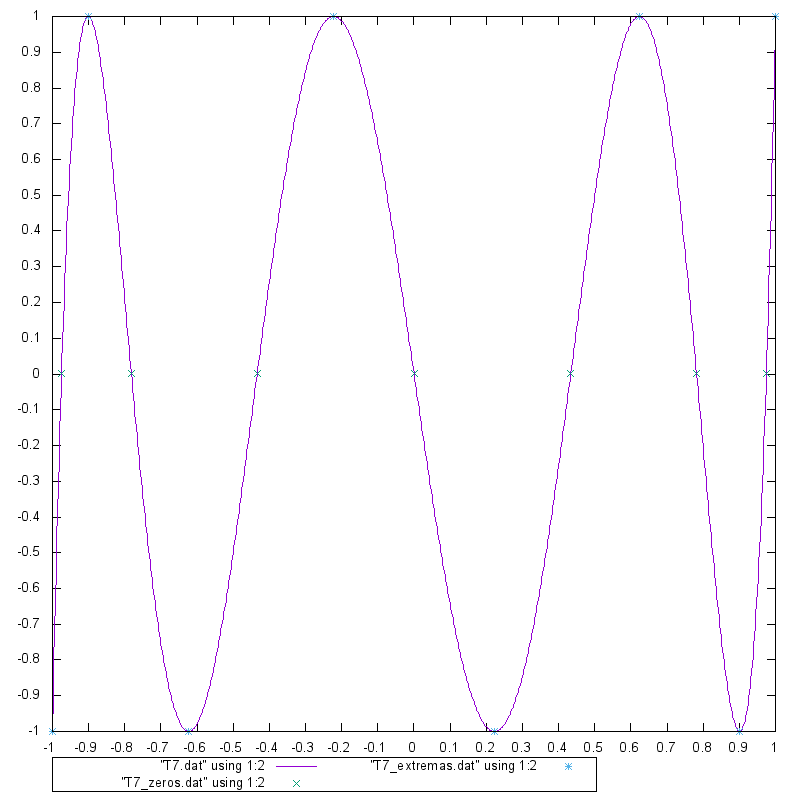
\includegraphics[scale=0.6]{T7}
\newline
Na het berekenen blijkt dat we best onze grafiek weergeven op het interval $[-1, 1]$. Hieronder de uit formules berekende x-waarden van nulpunten en extrema:
\newline

\begin{tabular}{ l c c r}
  j & Nulpunt & Extrema(x) & Extrema(y) \\
  0 & / & 1 & 1 \\
  1 & 0.974928 &0.900969 & -1  \\
  2 & 0.781831 & 0.62349 & 1 \\
  3 & 0.433884 & 0.222521 & -1 \\
  4 & 6.12323e-17 & -0.222521 & 1   \\
  5 & -0.433884 & -0.62349 & -1  \\
  6 & -0.781831 & -0.900969 &  1 \\
  7 & -0.974928 & -1 & -1  \\  
\end{tabular}
\newline
\newline

Wanneer we visueel de grafiek bestuderen lijken de formules uit de cursus correct! De berekende nulpunten liggen op de coördinaten waar de nulpunten van de grafiek liggen. Bij de berekende extrema is dit hetzelfde.

\section{Maak $T_{7}(x)$ monisch}
Een monische chebychev vergelijking wordt berekend door: $\frac{T_{n}(x)}{2^{n-1}}$ in het geval van $T_{7}(x)$ zal dit dus de veelterm $\frac{T_{7}(x)}{2^{6}}$ zijn.
\newline

We willen weten wat de bovengrens is van de absolute waarde van deze functie.We hebben een formule in de cursus voor het berekenen van extrema van een chebychev veelterm, deze is makkelijk aan te passen naar een versie die kan werken met de monische chebychev veelterm.
\newline

$  T_{i}(cos(\frac{j\pi}{i}) = \frac{ (-1)^{j} }{2^{i-1}} $ voor j = 0, ..., i
\newline

En dus voor $T_{7}(x)$
\newline

$  T_{7}(cos(\frac{j\pi}{7})  = \frac{ (-1)^{j} }{2^{6}} $ voor j = 0, ..., i
\newline

Wanneer we nu het programma geschreven voor het derde deel van deze oefening aanpassen met deze nieuwe veelterm en de absolute waarde functie krijgen we volgende extrema:
\newline

\begin{tabular}{ l c r }
  j & Extrema(X) & Extrema(Y) \\
  0 &  1 & 0.015625  \\
  1 & 0.900969 &  0.015625  \\
  2 &  0.62349 & 0.015625  \\
  3 & 0.222521 & 0.015625  \\
  4 & -0.222521 &  0.015625  \\
  5 & -0.62349 &  0.015625  \\
  6 & -0.900969 & 0.015625   \\
  7 &  -1 &  0.015625  \\  
\end{tabular}
\newline
\newline

Dit is niet verwonderlijk, de extrema zijn door de absolute waarde functie allemaal positief geworden. Door het monisch maken van de veelterm wordt elke y waarde van de functie gedeeld door 64 en dus ook de extrema. Waardoor we kunnen stellen dat de functie een bovengrens 0.015625 heeft.

\section{Code}
\textbf{T7.cpp} voor berekenen van deel 3

\lstinputlisting{T7.cpp}

\textbf{Monisch.cpp} voor berekenen van deel 4

\lstinputlisting{Monisch.cpp}

\end{flushleft}
\end{document}